%%%%%%%%%%%%%%%%%%%%%%%%%%%%%%%%%%%%%%%%%%%%%%%%%%%%%%%%%%%%%%%%%%%%%%%%%%%%%%%%
% Preámbulo                                                                    %
%%%%%%%%%%%%%%%%%%%%%%%%%%%%%%%%%%%%%%%%%%%%%%%%%%%%%%%%%%%%%%%%%%%%%%%%%%%%%%%%

\documentclass[11pt,a4paper,titlepage,oneside]{report}

%%% RELACIÓN DE VARIABLES A PERSONALIZAR %%%
% \def\lingua{gal}
\def\lingua{esp} % descomenta esta liña se redactarás a memoria en español
%\def\lingua{eng} % descomenta esta liña se redactarás a memoria en inglés
\def\nome{Mateo Tilves Freijeiro}                             % substitúe aquí o teu nome
\def\nomedirectorA{Juan Raposo Santiago}              % substitúe aquí o nome de quen dirixe
%\def\nomedirectorB{Outro Nome Completo}             % duplica esta liña máis veces se o precisas, cambiando
                                                     % a letra final (A, B, C, D...): úsanse na portada.tex
\def\titulo{Aplicación para axudar na xestión e monitorización das vendimias
} % substitúe aquí o título do teu TFG
%\def\titulacion{gced}                               % descomenta esta liña e comenta a seguinte se es estudante do GCED
\def\titulacion{gei}
%\def\mencion{COMPUTACIÓN}                           % descomenta a mención que che corresponda se es estudante do GEI
\def\mencion{ENXEÑARÍA DO SOFTWARE}
%\def\mencion{ENXEÑARÍA DE COMPUTADORES}
%\def\mencion{SISTEMAS DE INFORMACIÓN}
%\def\mencion{TECNOLOXÍAS DA INFORMACIÓN}

\def\renomearcadros{si} % descomenta esta liña se redactas a memoria en español e prefires que
                         % os "cuadros" e o "índice de cuadros" se renomeen
                         % a "tablas" e "índice de tablas" respectivamente

\usepackage{estilo_tfg}

% Lista de paquetes potencialmente interesantes (uso baixo demanda)

% \usepackage{alltt}       % proporciona o entorno alltt, semellante a verbatim pero que respecta comandos
% \usepackage{enumitem}    % permite personalizar os entornos de lista
% \usepackage{eurofont}    % proporciona o comando \euro
% \usepackage{float}       % permite máis opcións para controlar obxectos flotantes (táboas, figuras)
% \usepackage{hhline}      % permite personalizar as liñas horizontais en arrays e táboas
  \usepackage{longtable}   % permite construir táboas que ocupan máis dunha páxina
% \usepackage{lscape}      % permite colocar partes do documento en orientación apaisada
% \usepackage{moreverb}    % permite personalizar o entorno verbatim
  \usepackage{multirow}    % permite crear celdas que ocupan varias filas da mesma táboa
% \usepackage{pdfpages}    % permite insertar ficheiros en PDF no documento
% \usepackage{rotating}    % permite diferentes tipos de rotacións para figuras e táboas
% \usepackage{subcaption}  % permite a inclusión de varias subfiguras nunha figura
% \usepackage{tabu}        % permite táboas flexibles
% \usepackage{tabularx}    % permite táboas con columnas de anchura determinada

%%%%%%%%%%%%%%%%%%%%%%%%%%%%%%%%%%%%%%%%%%%%%%%%%%%%%%%%%%%%%%%%%%%%%%%%%%%%%%%%
% Corpo                                                                        %
%%%%%%%%%%%%%%%%%%%%%%%%%%%%%%%%%%%%%%%%%%%%%%%%%%%%%%%%%%%%%%%%%%%%%%%%%%%%%%%%

\begin{document}

 %%%%%%%%%%%%%%%%%%%%%%%%%%%%%%%%%%%%%%%%
 % Preliminares do documento            %
 %%%%%%%%%%%%%%%%%%%%%%%%%%%%%%%%%%%%%%%%

 \begin{titlepage}
  
  \hspace*{128pt}
  \textcolor{udcpink}{{\fontencoding{T1}\fontfamily{phv}\selectfont Facultade de Informática}}\\[-32pt]

  \begin{center}
    
\includegraphics[scale=0.3]{imaxes/udc}\\[25pt]

    {\large TRABALLO FIN DE GRAO \\
            \nometitulacion \\
            \nomemencion } \\[10pt]

    \carimbo \\[25pt]

    \begin{huge}
      \begin{spacing}{1.3}
        \bfseries \titulo
      \end{spacing}
    \end{huge}
  \end{center}
  
  \vfill
  
  \begin{flushright}
    {\large
    \begin{tabular}{ll}
      {\bf Estudante:} & \nome \\
      {\bf Dirección:} & \nomedirectorA \\
%                      & \nomedirectorB \\ % duplica esta liña máis veces se o precisas, cambiando
                                           % a letra final (A, B, C, D...); define eses nomes no memoria_tfg.tex
    \end{tabular}}
  \end{flushright}
  \rightline{A Coruña, \datasimple.}
\end{titlepage}

 \dedicatoria{} % escribe neste comando o teu texto de dedicatoria
 \paxinaenbranco
 \begin{agradecementos}
 % substitúe este comando polo teu texto de agradecementos
 \end{agradecementos}
 %%%%%%%%%%%%%%%%%%%%%%%%%%%%%%%%%%%%%%%%%%%%%%%%%%%%%%%%%%%%%%%%%%%%%%%%%%%%%%%%

\pagestyle{empty}
\begin{abstract}
    
  El trabajo consiste en el diseño, implementación de una aplicación para ayudar en la gestión de
  procesos de negocio de una empresa viticultora, en específico en el proceso de la recogida de la uva
  (vendimia).

  Durante el proceso de vendimia la plantilla de empleados crece enormemente por lo que una
  aplicación para la ayuda de la gestión de los trabajos de los empleados puede ayudar mucho en el
  control y trazabilidad de la uva y del trabajo realizado.

  La aplicación tendrá un catálogo de zonas de recogida y líneas de parras asociadas a cada zona, y
  estas líneas de parras con datos sobre el tipo de uva, el tipo de formación empleados en la línea,
  edad, metros de línea, etc. Esta información podrá ser creada y modificada por empleados de la
  empresa con rol de administrador.Para la gestión del trabajo de la vendimia, los capataces podrán, mediante el uso de la aplicación,
  informar del trabajo realizado en las distintas líneas de parras, tanto de tareas de mantenimiento
  previa a la vendimia, como de la recogida de la uva.

  Los tractoristas tendrán un rol especial, ya que serán notificados una vez se trabaje por completo una
  cantidad determinada de líneas de parras, con información detallada de la zona y líneas que deben
  recoger.

  Para la facilidad de uso de la aplicación por parte de los capataces, estos podrán registrar el trabajo
  de cada línea de parras con un código QR, que habrá en cada línea de parras.

  Los capataces podrán utilizar la aplicación para añadir trabajos asociados a cada una de las líneas de
parras, asignando recursos (personal de vendimia), tipo de trabajo, y opcionalmente añadir
comentarios sobre el trabajo realizado en una línea de parras. Para facilitar el uso se puede leer un
código QR para iniciar este proceso, aunque también tendrá la posibilidad de buscar la zona y línea
manualmente.

Habrá tres tipos de roles; administrador, capataz y tractoristas. Un mismo usuario podrá ejercer rol
de capataz y tractorista. Se requerirá autenticación de estos usuarios.
La aplicación constará de un backend y un frontend. El backend estará implementado en Java, y será
accesible mediante una API REST basada en Spring y desarrollada con una metodología API First con
el uso de la herramienta OpenAPI.



\vspace*{25pt}
\begin{segundoresumo}
  
  The work consists in the design and implementation of an application to help in the management of
  business processes of a wine-growing company, specifically in the process of grape harvesting (grape harvest).

  During the harvesting process, the number of employees grows enormously, so an application for the
  application to help manage the work of the employees can be of great help in the control and traceability of the grapes.
  control and traceability of the grapes and the work carried out.

  The application shall have a catalogue of harvesting zones and vine lines associated to each zone, and
  these vine lines with data on the type of grape, the type of formation used on the line, age, metres of line, etc. 
  This information can be created and modified by company employees with the role of administrator.
  For the management of harvest work, foremen will be able, by using the application, to report on the work carried out on the different lines,
  report on the work carried out on the different lines of vines, both in terms of maintenance tasks prior to the harvest, as well as
  tasks prior to the harvest, as well as grape harvesting.

  Tractor drivers will have a special role, as they will be notified once a certain number of vine lines have been completely worked.
  number of lines of vines are completely worked, with detailed information on the area and lines where to pick up the boxes loaded with grapes.

  For the ease of use of the application by the foremen, they will be able to register the work of each line of vines with a QR code, 
  which will be on each line of vines.

  Foremen will be able to use the application to add jobs associated with each of the lines of vines, 
  assigning resources (harvesting personnel, type of work, and optionally adding
  resources (harvesting personnel), type of work, and optionally add comments on the work carried out on a line of vines.
  comments on the work carried out on a line of vines. For ease of use, a
  QR code can be read to start this process, although you can also search for the area and line manually.
  
  There will be three types of roles; administrator, foreman and tractor drivers. The same user will be able to play the role of
  foreman and tractor driver. Authentication of these users will be required.
  The application will consist of a backend and a frontend. The backend will be implemented in Java, and it will be
  accessible via a REST API based on Spring and developed with an API First methodology using the OpenAPI tool.
\end{segundoresumo}
\vspace*{25pt}
\begin{multicols}{2}
  \begin{description}
  \item [\palabraschaveprincipal:] \mbox{} \\[-20pt]
    \begin{itemize}
      \item JPA
      \item Hibernate
      \item Spring
      \item Flutter
      \item OpenAPI
      \item OAS
      \item OpenAPI Generator
      \item Scrumban
      \item Funcionalidad
      \item Vendimia
      \item Administrador
      \item Capataz
      \item Tractorista 
    \end{itemize}
  \end{description}
  \begin{description}
  \item [\palabraschavesecundaria:] \mbox{} \\[-20pt]
    \begin{itemize}
      \item JPA
      \item Hibernate
      \item Spring
      \item Flutter
      \item OpenAPI
      \item OAS
      \item OpenAPI Generator
      \item Scrumban
      \item Feature
      \item Harvest
      \item Administrator
      \item Foreman
      \item Tractor driver
    \end{itemize}

  \end{description}
  \end{multicols}
  
\end{abstract}
\pagestyle{fancy}

%%%%%%%%%%%%%%%%%%%%%%%%%%%%%%%%%%%%%%%%%%%%%%%%%%%%%%%%%%%%%%%%%%%%%%%%%%%%%%%%


 \pagenumbering{roman}
 \setcounter{page}{1}
 \bstctlcite{IEEEexample:BSTcontrol}

 \tableofcontents
 \listoffigures
 \listoftables
 \clearpage
 
 \pagenumbering{arabic}
 \setcounter{page}{1}

 %%%%%%%%%%%%%%%%%%%%%%%%%%%%%%%%%%%%%%%%
 % Capítulos                            %
 %%%%%%%%%%%%%%%%%%%%%%%%%%%%%%%%%%%%%%%%

 \chapter{Introducción}
\label{chap:introducion}

% \lettrine{P}{rimer} capítulo da memoria, onde xeralmente se exporán as
% liñas mestras do traballo, os obxectivos, etc. Incluimos un par de
% exemplos de citas~\cite{ErlangBook,ErlangWebBook} e de referencias
% internas (sección \ref{sec:mostra}, páxina \pageref{sec:mostra}).

\lettrine{L}{a} vendimia es la recolección de la uva, que se procesa y se trata para obtener vino. 
Esta actividad milenaria se realiza normalmente en los meses de septiembre y octubre, cuando se recogen los frutos maduros de la vid.
Es un evento en el que se reúne mucha gente para "apañar" la uva, y motivo de festividad~\cite{Vendimia} en muchos puntos de Galicia(y del mundo).
Normalmente, en viñas domésticas no muy extensas, el trabajo es muy manual y no requiere de mucha gente y tiempo para la recolectar toda la uva.
Lo mas habitual es que hagan uso de un sistema de emparrado de conducción horizontal, l, típico en el rural gallego, especialmente en las Rías Baixas, 
donde las plantas de vids se forman con una estructura de pasillo de "arcos" ~\ref{fig:emparrado}. A pesar de su belleza en el rural, normalmente están construidos 
para la "comodidad" de cada dueño de la vid, por lo que puede ser difícil encontrar dos arcos a la misma altura. Esto hace que la recolección de la uva se mas difícil para personas de distinta altura 
y además dificulta el uso de maquinaria especifica como los tractores~\ref{fig:tractorEmparrado}.


  \begin{figure}[hp!]
    \centering
    \begin{subfigure}[c]{0.75\textwidth}
      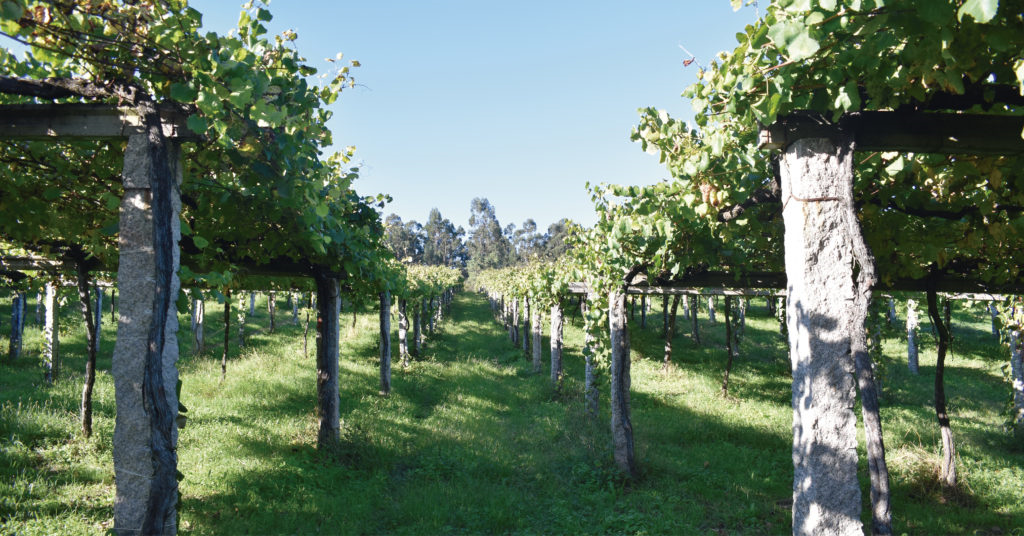
\includegraphics[width=\textwidth]{imaxes/sistema_emparrado.png}
      \caption{Formación vid emparrado}
      \label{fig:emparrado}
    \end{subfigure}
    \hspace{0.1\textwidth}
    \begin{subfigure}[c]{0.65\textwidth}
      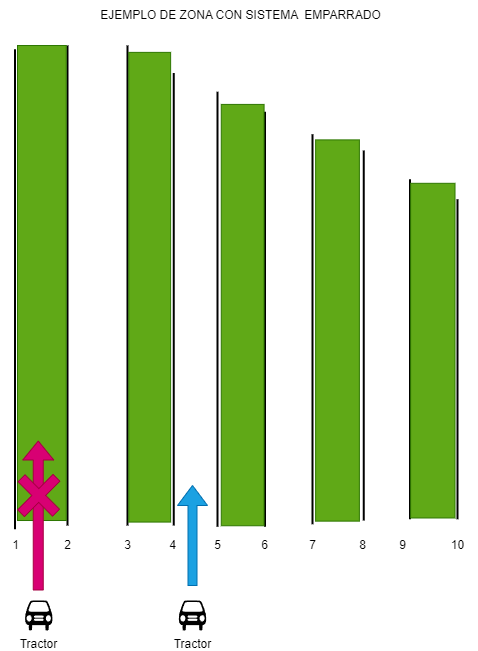
\includegraphics[width=\textwidth]{imaxes/2-EmparradoTractor.png}
      \caption{Maquinaria en emparrado}
      \label{fig:tractorEmparrado}
    \end{subfigure}
    \caption{Sistema de formación Emparrado}
    \label{fig:exemplo-subfiguras}
  \end{figure}
  
En empresas viticultoras con viñas extensas que recolectan muchas toneladas de uva, dependiendo del tamaño del terreno utilizado para el cultivo de las vides, 
el tipo de uva y su rendimiento ~\cite{RendimientoViticultura}.A pesar de que muchas empresas siguen teniendo vides en formación de emparrado horizontal, aprovechando así vides antiguas para la producción de vino de mayor calidad, 
se suele utilizar una formación de parras verticales, denominada formación espaldera ~\ref{fig:espaldera}. Esta formación en espaldera es mucho mas eficiente para trabajar, 
tanto para operarios de mantenimiento en tareas como podas, control de plagas y enfermedades, y el uso de maquinaria para tareas fitosanitarias, como para operarios de la vendimia, ya que la recolección es mucho mas sencilla 
y facilita el uso de maquinaria para la recogida de las cajas de uvas.~\ref{fig:tractorEspaldera}


\begin{figure}[hp!]
    \centering
    \begin{subfigure}[c]{0.75\textwidth}
      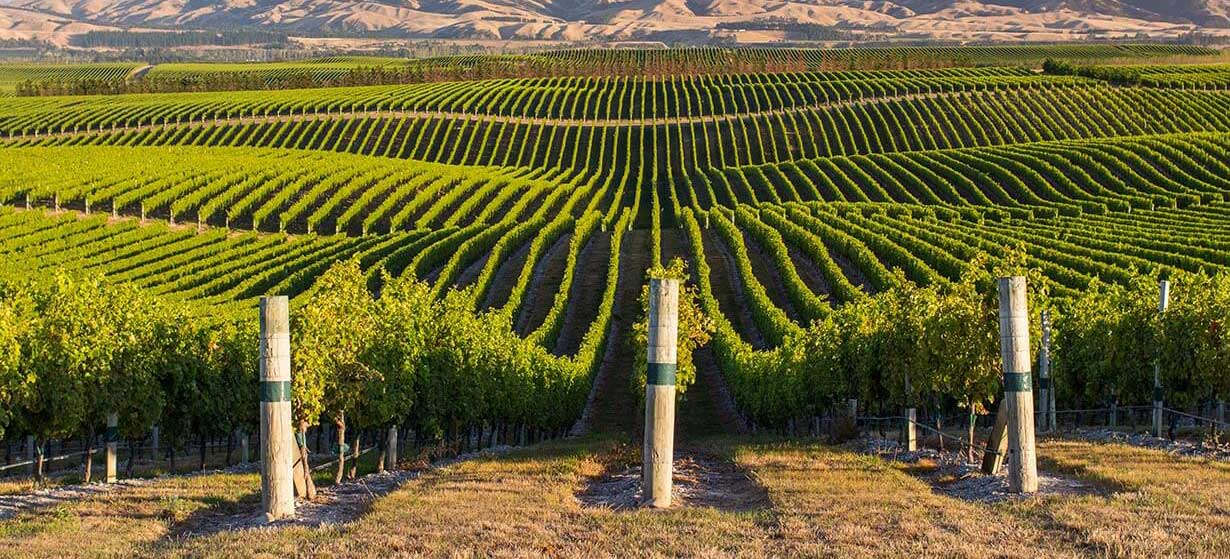
\includegraphics[width=\textwidth]{imaxes/3-Espalderas.png}
      \caption{Formación vid emparrado}
      \label{fig:espaldera}
    \end{subfigure}
    \hspace{0.1\textwidth}
    \begin{subfigure}[c]{0.65\textwidth}
      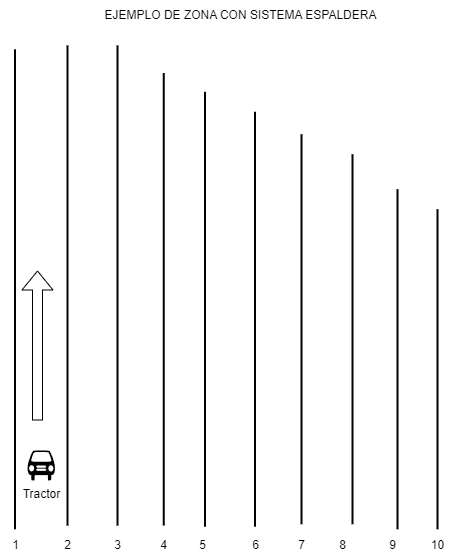
\includegraphics[width=\textwidth]{imaxes/4-EspalderasTractor.png}
      \caption{Maquinaria en emparrado}
      \label{fig:tractorEspaldera}
    \end{subfigure}
    \caption{Sistema de formación Espaldera}
    \label{fig:exemplo-subfiguras}
  \end{figure}


  Cada año en una empresa viticultora realiza una campaña para la vendimia. Esta campaña consiste en la ejecución de tareas específicas en todas las líneas de vides. 
  En concreto, el grupo de tareas esenciales en cada linea para la realización de una vendimia son las siguientes:
\begin{description}
  \item[Limpieza de las líneas:] Consiste principalmente en la limpieza de los pasillos entre dos lineas de vides para facilitar las siguientes tareas. 
  Normalmente, la tarea consiste en desbrozar, y suele ser personal propio de la empresa viticultora quien realiza esta tarea.

  \item[Poda de las líneas:] Consiste en podar las hojas y ramas que estorban y que pueden entorpecer el trabajo de la recolección. 
  En estas tareas trabajan conjuntamente capataces y personal de vendimia (personal externo) con experiencia previa.
  
  \item[Recolección de la uva:]
  La tarea más significativa para la vendimia. Consiste en el corte de los racimos de uva y su almacenamiento en cajas, 
  Estas cajas se llenan y se almacenan debajo de la estructura de la linea de la vid para facilitar la siguiente tarea de carga. 
  En estas tareas, solo el personal de vendimia trabajara en las líneas, mientras que los empleados de la empresa supervisan el trabajo realizado 
  (por lo que a partir de aquí denominare capataces a los empleados de las vids). Estas son las más criticas y demanda muchos recursos. 

  \item[Carga de las cajas de uva:] Durante esta tarea, un capataz con permiso de conducción de tractor, junto con, normalmente, tres personas más de personal de vendimia, 
  almacenarán las cajas de racimos de uva en el tractor, y cada vez que se llena el tractor o no queden cajas por recoger este será destinado a bodega donde se almacenaran los racimos de uva. Debe realizarse justo después de la recolección de la uva


\end{description}

\section{Motivación}

Durante el inicio de la campaña anual de la vendimia, comenzando con las tareas de limpieza, la empresa no necesita muchos cambios en la organización, ya que el propio personal de la empresa 
que realiza estas tareas. Sin embargo, a medida que avanza la campaña se incorpora mas gente, alcanzando el máximo en la tarea de recolección de la uva, 
por lo que la situación se vuelve caótica casi de un día para otro.
Durante la etapa de recolección pueden ocurrir numerosos incidentes que provoquen la pausa en la recogida de la uva, como climatología adversa que afecte a todas las líneas. 
Sin embargo, incidentes específicos en líneas individuales, como lesiones de los operarios, picaduras de avispas, golpes de calor o fatiga que impida la finalización de los trabajos asignados, también son situaciones comunes.
Evidentemente, los capataces atienden y socorren a los operarios de recolección en este tipo de situaciones. Sin embargo, después de atender a los operarios, 
a menudo pueden ocurrir desorganizaciones, como que el capataz  no recuerde la linea donde no se finalizo la recolección, cambios incorrectos en los turnos de capataces 
que resultan en confusión sobre qué líneas supervisar, o que los propios capataces enfrenten urgencias personales que los obliguen a abandonar su puesto.

Normalmente, el administrador gestiona el avance de la campaña de vendimia comunicándose con los capataces mediante llamadas y aplicaciones de mensajería instantánea.
Sin embargo, pueden ocurrir incidencias no notificadas que pueden llevar a una mala organización de los recursos y a un seguimiento deficiente del progreso de los trabajos en las lineas.

Por tanto, la creación de una aplicación móvil para ayudar en la organización de las tareas y en el control del progreso de las lineas seria beneficiosa. Esto facilitaría la coordinación tanto para los capataces como para los administradores.


\section{Objetivos}

Los principales objetivos con la realización del proyecto son, poner orden al caos con:
\begin{enumerate}
  \item Gestión de la información relativa a las lineas de vides, agrupadas por zonas. El administrador se encargara de decidir que lineas de vides son validas para su posterior recolección.
  \item Gestión de la los empleados de la empresa viticultora(capataces). El administrador se encarga de añadir a los capataces en el sistema, los cuales podrán hacer uso de la aplicación.
  \item Gestión de los operarios de vendimia. El administrador también es responsable de llevar un registro de la disponibilidad horaria de los operarios de vendimia, dado que puede variar considerablemente día a día. 
  Además, la aplicación permitirá tomar asistencia del personal de vendimia para eliminar su presencia del calendario en caso de ausencia ese mismo día, o incluso dar de baja de manera permanente.
  \item Gestión de las tareas de las líneas. Los capataces y los tractoristas son responsables de registrar el inicio de las tareas y de asignar los operarios de vendimia. 
  Además, serán ellos quienes registren la finalización de las tareas, incluyendo el porcentaje de avance y cualquier incidente ocurrido, permitiendo así un seguimiento completo de la vendimia.
  \item Idear funcionalidades que agilicen todo lo posible el proceso de seguimiento de las tareas.
\end{enumerate}

Además de los puntos anteriores, mis objetivos también son mejorar mis conocimientos de Spring Framework, iniciarme en el desarrollo de aplicaciones móviles con Flutter 
y documentarme y experimentar con la generación automática de código y documentación mediante el uso de la especificación OpenAPI.



% \Blindtext

% \section{Sección de mostra}
% \label{sec:mostra}

% \Blindtext

% \subsection{Subsección de mostra}

% \Blindtext

 \chapter{Tecnologías}
\label{chap:tecnologias}

\lettrine{E}{n} este capitulo expongo las tecnologías y herramientas utilizadas en la realización del proyecto.



\section{Lenguajes de programación}
% Se explica brevemente que lenguajes uso y el motivo por el que los elegí.
    \subsection{JPQL}
    Jakarta Persistence Query Languaje(anteriormente Java Persistence Query Languaje)~\cite{JPQL} es un lenguaje simple, basado en cadenas, similar a SQL, y que se utiliza para consultar entidades y sus relaciones.
    \subsection{Java}
    Java es un lenguaje de programación basado en clases y orientado a objetos. El motivo por el cual elegí este lenguaje es por la familiaridad con el mismo.
    \subsection{Yaml}
    YAML~\cite{YAML} es un lenguaje de serialización de datos diseñado para ser leído y escrito por humanos. Uso este lenguaje para crear archivos de configuración y especificación.
    \subsection{Dart}
    Dart~\cite{Dart} es un lenguaje de programación orientado a objetos y de código abierto desarrollado por Google. Este lenguaje porque es el lenguaje de las aplicaciones de Flutter.
    \subsection{Moustache}
    Moustache~\cite{Moustache} es un lenguaje para la creación de sistemas de plantillas. En concreto lo usare para la modificación de configuraciones. 

\section{Librerías y/o Frameworks}
    \subsection{Spring Framework}
    Spring Framework~\cite{Spring} es un marco de trabajo para el desarrollo de aplicaciones Java, que proporciona infraestructura para la gestión de dependencias, 
    programación orientada a aspectos, seguridad, y soporte para aplicaciones web. Facilita la creación de aplicaciones robustas y escalables mediante su enfoque modular y su amplia gama de componentes integrados.
    Permite el uso de sus módulos, los cuales facilitan la construcción de la capa modelo y capas de controlador de la interfaz web. Las características mas importantes que ofrece Spring Framework en este proyecto son:
    \begin{description}
        \item[Inversión de Control (IoC)]: Gestiona las dependencias de los objetos mediante la inyección de dependencias, facilitando la creación de aplicaciones desacopladas y más fáciles de probar.
        \item[Acceso a Datos Simplificado]: Proporciona integración simplificada con diversas tecnologías de acceso a datos, como JDBC, JPA y Hibernate, a través de plantillas y abstracciones.
        \item[Desarrollo de Aplicaciones Web]: Ofrece un robusto marco MVC (Model-View-Controller) para el desarrollo de aplicaciones web, incluyendo soporte para RESTful web services y WebSocket.
    \end{description}
    \subsection{OpenAPI Specification/OAS}
    La especificación OpenAPI~\cite{OpenAPI}, anteriormente conocido como Swagger, que permite describir, producir, consumir y visualizar APIs HTTP.
    Esta especificación, que se describe en formato YAML o JSON, se usa para crear documentación automática de estas APIs y puede incluso mediante el uso la herramienta
    OpenAPI Generator nos permite el generar librerías de código con las que podremos dar uso tanto en lenguaje servidor como cliente.
    \subsection{Flutter}
    Flutter ~\cite{Flutter} es un framework de código abierto creado por Google para desarrollar aplicaciones nativas multiplataforma desde una única base de código. 
    Utiliza el lenguaje de programación Dart y permite la creación de aplicaciones móviles, web y de escritorio con alto rendimiento y interfaces de usuario personalizables.
\section{Herramientas}
    \subsection{Organización}
        \subsubsection{Taiga}
        Taiga ~\cite{Taiga} es una herramienta gratuita y de código abierto orientada a la gestión de proyectos kaban y scrum.
    \subsection{Diseño}
        \subsubsection{PlantUML}
        PlantUML~\cite{Plantuml} es un componente que permite crear diagramas UML a través de descripciones textuales simples. PlantUML provee una forma fácil de crear representaciones visuales de sistemas complejos.
        \subsubsection{Figma}
        Figma~\cite{Figma} es una herramienta de generación de prototipos. Se usara esta herramienta para la creación de prototipos de las pantallas del aplicativo móvil.
    \subsection{Bases de datos}
        \subsubsection{H2}
        H2~\cite{H2} es una base de datos de Java en memoria y muy liviana, con una interfaz fácil de utilizar en navegador. Se utilizara esta base de datos para el desarrollo de la aplicación.
        \subsubsection{MySQL}
        MySQL~\cite{MySQL} es una base de datos relacional de código abierto, es una de las mas populares gracias a su facilidad de uso, rendimiento y fiabilidad. Esta base de datos seria la utilizada en un entorno de producción.
    \subsection{Entornos de desarrollo(IDEs)}
        \subsubsection{IntelliJ IDEA}
        IntelliJ IDEA~\cite{IDEA} es un entorno de desarrollo creado por JetBrain para el desarrollo software, especialmente enfocado en el desarrollo de aplicaciones Java, pero también tiene soporte para otros lenguajes de programación.
        \subsubsection{Android Studio}
        Android Studio~\cite{Android} es un entorno de desarrollo oficial de aplicaciones Android. Basado en IntelliJ IDEA, pero con muchas mas funciones para la productividad del desarrollo móvil. También tiene soporte para el desarrollo de aplicaciones móviles con Flutter.
    \subsection{Control de versiones}
        \subsubsection{Github}
        Github~\cite{Github} plataforma de desarrollo colaborativo basada en Git~\cite{Git}. Permite gestionar y compartir código, colaborar en proyectos, realizar seguimientos de cambios y revisar ramas mediante pull requests.
        Además se hace uso de Github Actions para la realización de pruebas de integración e inspección continua.

    \subsection{Docker}
    Docker~\cite{Docker} es una plataforma de contenedorización que permite a los desarrolladores empaquetar aplicaciones y sus dependencias en contenedores portátiles y ligeros. 
    Estos contenedores pueden ejecutarse de manera consistente en cualquier entorno, facilitando el despliegue y la escalabilidad de aplicaciones.

% \Blindtext

 \chapter{Contido demostrativo}
\label{chap:demo}

\lettrine{E}{ntre} a introdución e as conclusións, o documento conterá
tantos capítulos como sexa preciso, sempre con coidado de non rebasar
o límite de 80 páxinas fixado polo regulamento de TFGs.

Empregaremos éste de xeito demostrativo, para ilustrar o uso de
elementos habituais que poidan ser de utilidade\footnote{Por exemplo,
  isto é unha nota a pé de páxina.}.

\section{Inclusión de imaxes}

Se precisamos imaxes no noso documento, incluirémolas do xeito que se
indica na figura~\ref{fig:exemplo} (páxina~\pageref{fig:exemplo}). Se
o facemos así, \LaTeX ubicará cada imaxe no mellor lugar posible,
lugar que pode variar a medida que o documento vaia crecendo coa
inclusión de máis texto e outros elementos (máis imaxes, táboas,
etc.).

\begin{figure}[hp!]
  \centering
  
\includegraphics[width=0.75\textwidth]{imaxes/udc.png}
  \caption{Pé de imaxe descritivo}
  \label{fig:exemplo}
\end{figure}

Recoméndase almacenar os ficheiros gráficos no directorio
\texttt{imaxes}.

\subsection{Inclusión de varias sub-imaxes}

Se precisamos inserir imaxes relacionadas, pode ser apropiado
incluílas como sub-figuras, do xeito que se pode apreciar na
figura~\ref{fig:exemplo-subfiguras} coas
imaxes~\ref{fig:subfigura-rotada}
e~\ref{fig:subfigura-deformada}. Como se pode ver nos exemplos desta
sección, sempre é recomendable referirse ás imaxes pola súa
referencia, xa que dese xeito non dependemos de onde queden ubicados
os elementos en cuestión.

\begin{figure}[hp!]
  \centering
  \begin{subfigure}[c]{0.3\textwidth}
    
\includegraphics[angle=45,width=\textwidth]{imaxes/udc.png}
    \caption{Pé de subimaxe rotada}
    \label{fig:subfigura-rotada}
  \end{subfigure}
  \hspace{0.1\textwidth}
  \begin{subfigure}[c]{0.3\textwidth}
    
\includegraphics[width=\textwidth,height=3cm]{imaxes/udc.png}
    \caption{Pé de subimaxe deformada}
    \label{fig:subfigura-deformada}
  \end{subfigure}
  \caption{Pé de imaxe xeral}
  \label{fig:exemplo-subfiguras}
\end{figure}

\clearpage

\section{Inclusión de táboas}

Se precisamos táboas no noso documento, incluirémolas do xeito que se
indica na táboa~\ref{tab:exemplo} (páxina~\pageref{tab:exemplo}). Se
o facemos así, \LaTeX ubicará cada táboa no mellor lugar posible,
lugar que pode variar a medida que o documento vaia crecendo coa
inclusión de máis texto e outros elementos (máis imaxes, táboas,
etc.).

\begin{table}[hp!]
  \centering
  \rowcolors{2}{white}{udcgray!25}
  \begin{tabular}{c|c}
  \rowcolor{udcpink!25}
  \textbf{Título de columna} & \textbf{Outro título de columna} \\\hline
  \textit{Título de fila} & Contido de celda \\
  \textit{Título de fila} & Contido de celda \\
  \textit{Título de fila} & Contido de celda \\
  \textit{Título de fila} & Contido de celda \\
  \textit{Título de fila} & Contido de celda \\
  \textit{Título de fila} & Contido de celda \\
  \end{tabular}
  \caption{Pé de táboa descritivo}
  \label{tab:exemplo}
\end{table}

Para táboas longas que ocupan varias páxinas, como é o caso da \ref{tab:longa},
recoméndase o uso do paquete \texttt{lontable}, descomentando a liña
correspondente no ficheiro raíz do proxecto (\verb+memoria_tfg.tex+).

\rowcolors{2}{white}{udcgray!25}
\begin{longtable}{l|r|c}
  \caption{Pé descritivo dunha táboa longa}
  \label{tab:longa} \\

  \rowcolor{udcpink!25}
  \textbf{Primeira columna} & \textbf{Segunda columna} & \textbf{Terceira columna} \\\hline
  \endfirsthead

  \multicolumn{3}{c}{\tablename\ \thetable{} -- {\small \textit{(vén da páxina anterior)}}} \\
  \rowcolor{udcpink!25}
  \textbf{Primeira columna} & \textbf{Segunda columna} & \textbf{Terceira columna} \\\hline
  \endhead

  \multicolumn{3}{c}{\dotfill{\small \textit{(continúa na páxina seguinte)}}\dotfill} \\
  \endfoot

  \endlastfoot

  Texto de exemplo & abcdef ghjijklmn & 123.456778 \\
  Texto de exemplo & abcdef ghjijklmn & 123.456778 \\
  Texto de exemplo & abcdef ghjijklmn & 123.456778 \\
  Texto de exemplo & abcdef ghjijklmn & 123.456778 \\
  Texto de exemplo & abcdef ghjijklmn & 123.456778 \\
  Texto de exemplo & abcdef ghjijklmn & 123.456778 \\
  Texto de exemplo & abcdef ghjijklmn & 123.456778 \\
  Texto de exemplo & abcdef ghjijklmn & 123.456778 \\
  Texto de exemplo & abcdef ghjijklmn & 123.456778 \\
  Texto de exemplo & abcdef ghjijklmn & 123.456778 \\
  Texto de exemplo & abcdef ghjijklmn & 123.456778 \\
  Texto de exemplo & abcdef ghjijklmn & 123.456778 \\
  Texto de exemplo & abcdef ghjijklmn & 123.456778 \\
  Texto de exemplo & abcdef ghjijklmn & 123.456778 \\
  Texto de exemplo & abcdef ghjijklmn & 123.456778 \\
  Texto de exemplo & abcdef ghjijklmn & 123.456778 \\
  Texto de exemplo & abcdef ghjijklmn & 123.456778 \\
  Texto de exemplo & abcdef ghjijklmn & 123.456778 \\
  Texto de exemplo & abcdef ghjijklmn & 123.456778 \\
  Texto de exemplo & abcdef ghjijklmn & 123.456778 \\
  Texto de exemplo & abcdef ghjijklmn & 123.456778 \\
  Texto de exemplo & abcdef ghjijklmn & 123.456778 \\
  Texto de exemplo & abcdef ghjijklmn & 123.456778 \\
  Texto de exemplo & abcdef ghjijklmn & 123.456778 \\
  Texto de exemplo & abcdef ghjijklmn & 123.456778 \\
  Texto de exemplo & abcdef ghjijklmn & 123.456778 \\
  Texto de exemplo & abcdef ghjijklmn & 123.456778 \\
  Texto de exemplo & abcdef ghjijklmn & 123.456778 \\
  Texto de exemplo & abcdef ghjijklmn & 123.456778 \\
  Texto de exemplo & abcdef ghjijklmn & 123.456778 \\
  Texto de exemplo & abcdef ghjijklmn & 123.456778 \\
  Texto de exemplo & abcdef ghjijklmn & 123.456778 \\
  Texto de exemplo & abcdef ghjijklmn & 123.456778 \\
  Texto de exemplo & abcdef ghjijklmn & 123.456778 \\
  Texto de exemplo & abcdef ghjijklmn & 123.456778 \\
  Texto de exemplo & abcdef ghjijklmn & 123.456778 \\
  Texto de exemplo & abcdef ghjijklmn & 123.456778 \\
  Texto de exemplo & abcdef ghjijklmn & 123.456778 \\
  Texto de exemplo & abcdef ghjijklmn & 123.456778 \\

\end{longtable}


\section{Inclusión de código fonte}

Se precisamos incluír fragmentos de código fonte, podemos facelo, por exemplo, da
seguinte maneira:

\begin{lstlisting}[language=C]
#include <stdio.h>
#define N 10

int main()
{
  int i;

  // Isto é un comentario
  puts("Ola, mundo!");

  for (i = 0; i < N; i++)
  {
    puts("LaTeX é a ferramenta de edición ideal para profesionais da informática!");
  }

  return 0;
}
\end{lstlisting}

\section{Uso da relación de acrónimos e do glosario}

Os acrónimos edítanse no ficheiro \texttt{bibliografia/acronimos.tex}
e úsanse empregando a orde \texttt{acrlong} para obter o termo
completo (deste xeito: \acrlong{erlang}), a orde \texttt{acrshort}
para obter o acrónimo (deste xeito: \acrshort{erlang}). A primeira vez
que usamos un termo con acrónimo no documento é recomendable usar orde
\texttt{acrfull} (que produce ambas versións á vez:
\acrfull{erlang}). Os acrónimos que non se usan no documento, non
aparecen na relación que se xerar na versión PDF.

Pola súa banda, os termos do glosario edítanse no ficheiro
\texttt{bibliografia/glo\-sa\-rio.tex} e úsanse empregando a orde
\texttt{gls} (deste xeito, \gls{bytecode}) ou \texttt{Gls} (deste
xeito, \Gls{bytecode}). Ao igual que os acrónimos, os termos que non
se usan no documento, non aparecen na relación que se xera na versión
PDF.

%\include{contido/...}
 \chapter{Conclusións}
\label{chap:conclusions}

\lettrine{D}{erradeiro} capítulo da memoria, onde se presentará a
situación final do traballo, as leccións aprendidas, a relación coas
competencias da titulación en xeral e a mención en particular,
posibles liñas futuras,\dots

\Blindtext


 %%%%%%%%%%%%%%%%%%%%%%%%%%%%%%%%%%%%%%%%
 % Apéndices, glosarios e bibliografía  %
 %%%%%%%%%%%%%%%%%%%%%%%%%%%%%%%%%%%%%%%%

 \appendix
 \appendixpage
 \chapter{Material adicional}
\label{chap:adicional}

\lettrine{E}{xemplo} de capítulo con formato de apéndice, onde se pode
incluír material adicional que non teña cabida no corpo principal do
documento, suxeito á limitación de 80 páxinas establecida no
regulamento de TFGs.

\Blindtext

%\include{anexos/...}

 \printglossary[type=\acronymtype,title=\nomeglosarioacronimos]
 \printglossary[title=\nomeglosariotermos]

 \bibliographystyle{IEEEtranN}
 \bibliography{\bibconfig,bibliografia/bibliografia}
 \clearpage
 
\end{document}

%%%%%%%%%%%%%%%%%%%%%%%%%%%%%%%%%%%%%%%%%%%%%%%%%%%%%%%%%%%%%%%%%%%%%%%%%%%%%%%%
